\chapter{Review of Related Literature}

	Over the years, different types of models have been developed for shelter location-allocation to support evacuation efforts, each with distinct objectives and often integrated with programming. This chapter delves into key theories in modeling and system integration that inform the development of effective shelter location-allocation systems. Moreover, comprehensive review of related literature is conducted, analyzing and synthesizing existing studies to highlight their relevance, explore the current models, and identify areas where system features are lacking. 

\section{Theoretical Framework}
	The development of the shelter location-allocation system draws on key theories which feature the optimization of shelter location-allocation, development, and assessment of the system.

\subsection{Operations Research}
 	Mathematical modeling is an approach to represent a real-life problem and solving them using mathematical techniques such as the operations research. This theory addresses the optimization of objectives, crucial in shelter location-allocation where factors like distance and cost must be balanced. The problem is modeled to find the optimal locations while minimizing travel distances and associated costs, making it ideal for a multi-objective optimization.

\subsection{Theory of Evolution}
	Inspired by Charles Darwin’s theory of evolution, evolutionary algorithms such as genetic algorithms simulate natural selection within code to solve complex optimization problems effectively. This approach is widely used due to its robustness and adaptability, and it will be applied to solve the multi-objective model for shelter location-allocation.

\subsection{Decision Theory}
 	Decision theory is a study of having a rational choice by using models and tools. This involves creating a system that serves as a decision support tool for decision-makers, such as the DRRMO, in allocation of shelters. It features user-defined parameters for model customization and provides functionality for creating, reading, updating, and deleting data.

\subsection{Software Product Assessment Framework (ISO 25010)}
	ISO 25010 provides standards for assessing software quality, covering aspects such as functionality, usability, reliability, and efficiency. This framework will guide the evaluation of our decision support system through surveys, ensuring it meets high-quality standards.

\section{Bulacan is vulnerable in disasters}
	One of the most devastating typhoons to hit the Philippines was Typhoon Ondoy. According to Managhaya's report, it claimed nearly 100 lives and affected around 250,000 families. Large parts of Luzon suffered significant damage, including Bulacan, resulting in heavy flooding. \parencite{James2009}

	According to a report by Reyes-Estrope covering Typhoon Fabian in 2021 \parencite{Carmela2021}, heavy rainfall caused by the southwest monsoon and Typhoon Fabian resulted in flooding across 35 villages in Bulacan, including Calumpit. The water level of the Angat Dam rose to 185.72 meters above sea level during this event. Moreover, Gozum's report on Typhoon Egay in 2023 \parencite{Iya2023} emphasizes the hardships faced by flood victims in Bulacan. The province was declared under a state of calamity due to Typhoon Egay, which affected over 200,000 families and forced many residents to evacuate.

\section{Existing shelter location-allocation models}
	The allocation of different resources during each evacuation phase is critical, however, this is often delayed, either due to extenuating circumstances or simply lack of a system. Therefore, optimization is a must. In this section, the paper will introduce different models with varying solving techniques to solve each of their own objectives.
	
	In disaster management, the organization of effective evacuation is important. \textcite{Yiying2022} address the challenge of determining optimal shelter locations and evacuation routes, integrating methods such as the normal distribution, analytic hierarchy process (AHP), and ordered weighted aggregation operator (OWA); These approaches that have assigned subjective scores and initial weights to critical attributes significantly advances shelter location models for disaster response.
	
	Different studies also features levels of shelters which introduces a hierarchy of shelters, each with different needs that they fulfill and with various requirements to be assigned a level. Therefore the levels of each shelter must be taken into account, and this segment of system requires the use of hierarchical optimization.
	
	\textcite{Yunjia2019} show the importance of site selection models in disaster scenarios, particularly highlighting the application of bilevel programming, a hierarchical optimization method first introduced by H.v. Stackelberg in 1934. The methods used are applied to different complex location problems, such as the p-median and p-center problems, which are crucial for the distribution of resources during emergencies. 
	
	Building on the hierarchical approach, \textcite{Xiujuan2019} applied a hierarchical model for shelter location and evacuee allocation, distinguishing between emergency shelters (EMS) and long-term shelters (LTS). Combined with an optimization algorithm, their model facilitates the selection of EMS locations from a pool of candidates, ensuring the initial allocation of evacuees. Over time, evacuees transitioned from EMS to LTS in a structured and efficient manner, highlighting the practical advantages of hierarchical models in emergency management. 
	
	In a different study created by \textcite{Yunjia2019}, the paper exposes various models to best represent a shelter location-allocation problem, Single-Objective, Multi-Objective, and Hierarchical models. These were compared for the objectives that were maximized and minimized, and then introduced different algorithms that may be used to solve them.
	
	Locally, according to a published thesis in University of the Philippines(UP) Diliman, there exists 4 shelter location-allocation models; BNST, BST, BNT, and WORK models that are solved using binary genetic algorithms. These answer the optimization of allocation in shelters based on the cost, distance, workplace, and the hierarchy of shelter. This study was applied to the area of Talisay in Batangas using simulated data for shelter information.
	
	A study similar to the thesis has been published locally, however this study answers the optimization of COVID-19 vaccination site allocations\parencite{Kurt2021}. This study features assigning and identifying shelters to be a vaccination sites considering its distance across all barangay.

\section{Optimization Technique by Genetic Algorithm}
	Since the optimization of shelter location-allocation  requires multiple iterations to test and figure out what is truly optimal, one method of solving this is through the use of genetic algorithms.
	
	In a study created by \textcite{Mathew2012}, Genetic Algorithms are based on the concept of natural selection and evolves possible solutions through operators such as selection, crossover, and mutation. Iterative processes are essential for refining solutions over successive generations. Multi-Objective Genetic Programming (MOGP) emphasizes the importance of semantic diversity and that methods like Pivot Similarity Semantic-based Distance outperform traditional approaches by enhancing solution quality and diversity, according to a study by \textcite{Edgar2020}.
	
	Numerous published studies and theses highlights allocation models and solved by genetic algorithm. From UP Diliman, \textcite{LeahUP} solved their model using Binary Genetic Algorithm. Additionally, a study made by \textcite{Ahmed2020}  which proposes a Hybrid Genetic Algorithm (HGA) in optimizing multi-objective problems. \textcite{Yin2023} exposed formulation of shelter allocation models, and solved by using Improved Quantum Genetic Algorithm (IQGA). 
	

\section{Lack of System Integration}
	The referenced articles each exposed models with various objectives. However, none offer a fully implemented system for practical use by disaster-response teams. This gap highlights the need for a comprehensive decision support system that integrates these models and enables real-time decision-making and adaptability in disaster situations. While the following articles propose a system, they remain incomplete and require further development.
	
	In the study of \textcite{Amir2023}, the researchers are claiming that the group has created a system, which features risk-based decision that affects the output. The paper, however, did not show the system structure nor the system itself. Moreover, they did not show any acceptability measures. \parencite{Amir2023}
	
	 The paper of \textcite{Cavdur2019} proposes the use of a decision support tool for the allocation of temporary disaster-response facilities while under the effects of demand uncertainty. The study also develops a database for storing disaster and shelter details to support disaster operations. This system closely aligns with this thesis, as it addresses shelter allocation and provides decision-making assistance for disaster-response teams. However, the study lacks any measures for evaluating system acceptability and has room for improvement, as the system design is also outdated.

\section{Synthesis of the Review}
	Overtime, the researchers have reviewed and analyzed multiple academic literature and studies that relate to the thesis. These range from literature and studies that cover different areas using differing allocation techniques as well as other formulae and algorithms that may be used in the thesis. However, a large amount of this literature and studies lack a system or other feature that is partly required for the usability of end-user. By studying these collected pieces of literature, the researchers aim to create a programmed system with enough improvements from the previous studies presented. Moreover, this thesis will base the models from the published paper from UP Diliman by \textcite{LeahUP}, with improved algorithm.

\section{Conceptual Framework}
	This section provides an Input-Process-Output framework (IPO) as a basis for conceptual framework outlining the development and implementation of Shelter Location-Allocation System for Calumpit, Bulacan. The IPO model was first introduced in the context of computer programming and documentation using the Hierarchy plus IPO (HIPO) technique. Moreover, the concept of input and output has been used before in economics, back in the 1930s, Wassily Leontief first conceptualized input-output analysis to illustrate economic interrelationships. Figure \ref{IPOModel} shows the IPO framework for this thesis.
	
	 \begin{figure}[h!]
		\centering
		\caption{IPO Model} \label{fig:ipo}
		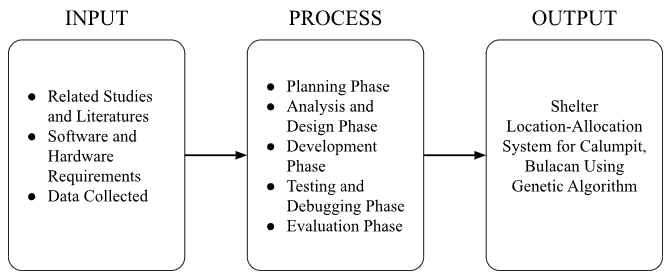
\includegraphics[width=\linewidth]{IPO}
		\label{IPOModel}
	\end{figure}
	
	The inputs for this project include related studies and literature, which provide a foundation for selecting and adapting an appropriate model for our system. These resources will be analyzed and synthesized to establish a strong foundation in conducting this project. We also need to gather software and hardware requirements, such as the compatible Windows version and system prerequisites, to ensure a smooth development process. Additionally, real data from Calumpit, Bulacan, specifically community and shelter information, will be essential for testing the system.
	
	The process begins with planning, where we outline the objectives and approach for building the system. Once a clear plan is established, we proceed to analysis and design, which involves creating mock-up designs, an ERD schema, and process flows to help developers visualize the system structure. Development phase is the longest phase, involving both frontend design and backend coding using the Qt framework. Once developed, the system undergoes rigorous testing to identify and correct any errors or anomalies, which will then be debugged and will be resolved. Finally, the system will be evaluated through a survey based on the ISO 25010 criteria to assess its acceptability.
	
	The expected output is a fully functional decision support system(DSS) that incorporates the  model adopted using a genetic algorithm as the solving method. The researchers will generate results showing the optimal shelter location-allocation for Calumpit using the developed system.
	


